\documentclass{beamer}
%\documentclass[handout]{beamer}

% Input all common stuff


% THEME SETTINGS %%%%%%%%%%%%
\usetheme[secheader]{Boadilla}
\usecolortheme{default}
\useinnertheme{circles}
\setbeamertemplate{blocks}[default]

% Get rid of bottom navigation bars
\setbeamertemplate{footline}[page number]{}

% Gets rid of navigation symbols
\setbeamertemplate{navigation symbols}{}

% PACKAGES %%%%%%%%%%%%%%%%%%%
\usepackage{listings}
\usepackage{xcolor}
\usepackage{multirow}
\usepackage{array}
\usepackage{verbatim}
\usepackage{pbox}
\usepackage{tabularx}

% LISTINGS STYLE %%%%%%%%%%%%%
\definecolor{bluekeywords}{rgb}{0.13,0.13,1}
\definecolor{greencomments}{rgb}{0,0.5,0}
\definecolor{redstrings}{rgb}{0.9,0,0}
\definecolor{listingsbg}{HTML}{EFEFFF}

\lstset{language=C++,
  showspaces=false,            % show spaces adding particular underscores
  showtabs=false,              % show tabs within strings adding particular underscores
  breaklines=true,             % sets automatic line breaking
  showstringspaces=false,      % underline spaces within strings
  breakatwhitespace=true,      % sets if automatic breaks should only happen at whitespace
  captionpos=b,                % sets the caption-position to bottom
  escapeinside={(*@}{@*)},
  commentstyle=\color{greencomments},
  keywordstyle=\color{bluekeywords}\bfseries,
  stringstyle=\color{redstrings},
  basicstyle=\ttfamily\fontsize{9}{10}\selectfont,
  backgroundcolor=\color{listingsbg}
}

% MACROS %%%%%%%%%%%%%%%%%%%%%
\newcommand{\lstsrctitle}[0]{%
 {\scriptsize\lstname}
}

\newcommand{\kw}[1]{\texttt{\textcolor{bluekeywords}{\ttfamily\fontsize{9}{10}\selectfont #1}}}

\newenvironment{varblock}[3]{%
  \setbeamercolor{block body}{#2}
  \setbeamercolor{block title}{#3}
  \begin{block}{#1}}{\end{block}}

% Colours taken from http://twitter.github.com/bootstrap/components.html#alerts
% Do block %%%%%%%%%%%%%%%%%%%%%%
\definecolor{doblocktext}{HTML}{468847}
\definecolor{doblockbg}{HTML}{DFF0D8}
\newenvironment{doblocke}[0]{% begin
  \begin{varblock}{\textbf{Do}}%
  {bg=doblockbg,fg=doblocktext}{bg=doblocktext,fg=white}%
  \setbeamercolor{itemize item}{fg=doblocktext}
  \lstset{backgroundcolor=}% The background should be the same as that of the block
  } % begin
  {\end{varblock}} %end
  
\newcommand{\doblock}[1]{%
 \begin{doblocke}#1\end{doblocke} 
}

% Don't block %%%%%%%%%%%%%%%%%%%
\definecolor{dontblocktext}{HTML}{B94A48}
\definecolor{dontblockbg}{HTML}{F2DEDE}  
\newenvironment{dontblocke}[0]{% begin
  \begin{varblock}{\textbf{Don't}}%
  {bg=dontblockbg,fg=dontblocktext}{bg=dontblocktext,fg=white}
  \setbeamercolor{itemize item}{fg=dontblocktext}
  \lstset{backgroundcolor=}% The background should be the same as that of the block
  }%
  {\end{varblock}} %end

\newcommand{\dontblock}[1]{%
 \begin{dontblocke}#1\end{dontblocke} 
}

% Defi block %%%%%%%%%%%%%%%%%%%%
\definecolor{defiblocktext}{HTML}{3A87AD}
\definecolor{defiblockbg}{HTML}{D9EDF7}
\newenvironment{defiblocke}[1]{% begin
  \begin{varblock}{\textbf{Definition}}%
  {bg=defiblockbg,fg=defiblocktext}{bg=defiblocktext,fg=white}
  \lstset{backgroundcolor=}% The background should be the same as that of the block
  \textit{#1} }
  {\end{varblock}} %end

\newcommand{\defiblock}[2]{%
 \begin{varblock}{\textbf{Definition}}%
 {bg=defiblockbg,fg=defiblocktext}{bg=defiblocktext,fg=white}%
  \begin{tabularx}{\linewidth}{lX}\textit{#1} & #2\end{tabularx}
 \end{varblock} 
}

\newenvironment{defiblockbaree}[1]{ %begin
  \begin{varblock}{\textbf{#1}}%
  {bg=defiblockbg,fg=defiblocktext}{bg=defiblocktext,fg=white}
  \lstset{backgroundcolor=}} %begin
  {\end{varblock}} %end

\definecolor{warnblocktext}{HTML}{C09853}
\definecolor{warnblockbg}{HTML}{FCF8E3}
\newenvironment{warnblocke}[0]{% begin
  \begin{varblock}{\textbf{Warning!}}%
  {bg=warnblockbg,fg=warnblocktext}{bg=warnblocktext,fg=white}
  \lstset{backgroundcolor=}% The background should be the same as that of the block
  \setbeamercolor{itemize item}{fg=warnblocktext}
  \setbeamercolor{item projected}{fg=white,bg=warnblocktext}
  } % begin
  {\end{varblock}} % end

\newcommand{\warnblock}[1]{%
  \begin{warnblocke}#1\end{warnblocke}
} % newcommand

\newcommand{\cout}[1]{%
 Output: \pbox[t]{\textwidth}{\ttfamily\fontsize{9}{10}\selectfont{}#1}
}

\newenvironment{doitemize}[0]{%
  \begin{itemize}}%
  {\end{itemize}} %end


% CONSTANTS %%%%%%%%%%%%%%%%%%%%%%%%%%%

%Symbol for backslash in texttt \char`\\

% Common title slide stuff
\title{Introduction to Scientific Programming with C++}
\author{Martin Uhrin}
\institute{UCL}
\date{February 11-13th 2013}

\usepackage{pifont}

\subtitle{Session 5: Advanced object oriented programming}

\begin{document}

\frame{\titlepage}

\begin{frame}
\frametitle{Table of Contents}
\tableofcontents
\end{frame}

\section{Class method definition}

\begin{frame}[fragile]
  \frametitle{Separating class definition and declaration}
 
  \begin{columns}[t]
    \begin{column}[T]{0.5\linewidth}
  		Often it's a pain to write the body of a function within the class, consider:
  		\begin{lstlisting}
class GameObject {
public:
  void draw()  {
  // many hundreds of lines
  // of graphics code here
  }
};
  		\end{lstlisting}
  		the class interface gets lost in all the graphics code.
  	\end{column}
  	\pause
  	\begin{column}[T]{0.5\linewidth}
  		To help with this we can write:
		  \begin{lstlisting}
class GameObject {
public:
  void draw();
};

// many lines or a
// different file later

GameObject::draw() {
  // many hundreds of lines
  // of graphics code here
}
  		\end{lstlisting}
  	\end{column}
  \end{columns}
  \pause
  This supports encapsulation by separating the interface from the implementation.  You'll often find declaration in a \texttt{.h} file and the definition in a \texttt{.cpp} file.

\end{frame}

\section{Inheritance}

\subsection{Single inheritance}

\begin{frame}
  \frametitle{Class inheritance}
  \framesubtitle{Not compatible with egalitarianism}

	Consider the following class:
  \lstinputlisting[language=C++,%
    basicstyle=\ttfamily\fontsize{8}{9}\selectfont,%
    linerange={4-19}]%
    {../code/5_advanced_oop/lectures/inheritance.cpp}
    \pause
  What if we want to create a dog class.  It can do everything a \texttt{Mammal} can.  It would be a shame to have to copy everything over.  With inheritance we don't have to!
\end{frame}

\begin{frame}
  \frametitle{Class inheritance}

  We can make a \texttt{Dog} inherit from \texttt{Mammal} like so:
  \lstinputlisting[language=C++,%
  	title=\lstsrctitle,belowskip=0pt,%
    linerange={54-65}]%
    {../code/5_advanced_oop/lectures/inheritance.cpp}
  \pause
  Now \texttt{Dog} has inherited members from \texttt{Mammal} so we don't have to rewrite them.  \texttt{Dog} is said to be \textit{derived} from \texttt{Mammal}. Makes sense, right?
\end{frame}

\begin{frame}[fragile]
  \frametitle{Class inheritance}
  \framesubtitle{Sit, boo-boo, sit.  Good dog.}
  
  This is what happens when we use the \texttt{Dog} class:
  \begin{columns}[t]
    \begin{column}[T]{0.5\linewidth}
  		\lstinputlisting[language=C++,%
  			title=\lstsrctitle,aboveskip=0pt,belowskip=0pt,%
    		firstline=86]%-102}
    		{../code/5_advanced_oop/lectures/inheritance.cpp}
    \end{column}
    \pause
  	\begin{column}[T]{0.48\linewidth}
  	  \cout{Fido is : 2 years old\newline
				and weighs 10 kg.\newline\newline
				Grrr, mammal noise!\newline
				\char`\\{}/\char`\\{}/\char`\\{}/ <- That's my tail wagging!\newline
				Fetching frisbee...Here you go.}
			  \begin{figure}
			    \centering
					\includegraphics[width=35mm]{figs/BostonTerrier.eps}
				\end{figure}
  	\end{column}
  \end{columns}

\end{frame}

\begin{frame}[fragile]
  \frametitle{Passing arguments to base constructors}
  
  \texttt{Mammal} has only one constructor:
  \lstinputlisting[language=C++,%
  	linerange={6-6}]%
  	{../code/5_advanced_oop/lectures/inheritance.cpp}
  So we need to give an age and a weight to build a \texttt{Mammal}.  Because \texttt{Dog} inherits from \texttt{Mammal} it too must provide these.\pause{} Here's how:
  \lstinputlisting[language=C++,%
  	linerange={67-73}]%
  	{../code/5_advanced_oop/lectures/inheritance.cpp}  
	The \texttt{Dog} class calls the \texttt{Mammal} constructor in the initialiser list as part of its constructor to initialise the \texttt{Mammal} part of itself.

\end{frame}

\begin{frame}[fragile]
  \frametitle{Initialiser lists}
  
	\defiblock{initialiser list}{a list used to initialise base class(es), class constants, member constants and (optionally) member variables as part of a class's constructor.}
	
	The format is:
	\begin{lstlisting}
  constructor_name(paramters...):
    initialise_item1,
    initialise_item2,
	  ...
	  { /* constructor body */ }
	\end{lstlisting}
	So we could also initialise a \texttt{Dog}'s breed in this list:
	\begin{lstlisting}
	Dog(const unsigned int age,
	  const unsigned int weight,
	  const std::string & breed):
	  myBreed(breed) {}
	\end{lstlisting}
\end{frame}

\begin{frame}[fragile]
  \frametitle{Overriding functions}
  
  When Fido spoke he said ``\texttt{Grrr, mammal noise!}'', not really what a Dog says.  That's because I didn't provide a custom \texttt{speak} method.  Let's try again:\pause
  \begin{columns}[t]
    \begin{column}[T]{0.55\linewidth}
  		\lstinputlisting[language=C++,%
  			title=\lstsrctitle,aboveskip=0pt,
  			linerange={54-55,62-63,67-67,86-95}]%
  			{../code/5_advanced_oop/lectures/inheritance2.cpp}  
  	\end{column}
  	\begin{column}[T]{0.4\linewidth}
  	  \cout{Woof!}
  	\end{column}
  \end{columns}
  \pause
  The new \texttt{speak} method is said to \textit{override} the one in \texttt{Mammal}.

\end{frame}

\begin{frame}[fragile]
  \frametitle{Derived class member access}
  
  Finally we get to see what the \kw{protected} access specifier is all about.  Access types can be summarised as follows:
  \begin{table}[h]
    \centering
	  \begin{tabularx}{0.75\linewidth}{l|c|c|c}
	    Access & \kw{public} & \kw{protected} & \kw{private} \\
	    \hline
	    members of same class & yes & yes & yes \\
	    members of derived class & yes & yes & no \\
	    non members & yes & no &  no
	  \end{tabularx}
  \end{table}
  \pause
  \doblock{Use the most restrictive access possible.  Member variables should rarely be anything but \kw{private}, even derived classes should use getters/setters to access these.  It's fine to make methods protected though.}
 
\end{frame}

\begin{frame}[fragile]
  \frametitle{What \textit{exactly} is inherited?}
  
  Pretty much everything is inherited by the derived class, except:
  \begin{itemize}
    \item{Constructors and destructors}
    \item{\texttt{operator =()} members}
    \item{friends (more on this later)}
  \end{itemize}

\end{frame}

\subsection{Multiple inheritance}

\begin{frame}[fragile]
  \frametitle{Multiple inheritance}
  
  Let's say we have the following classes:
  \begin{columns}[t]
    \begin{column}[T]{0.45\linewidth}
  		\begin{lstlisting}[aboveskip=0pt,belowskip=0pt]
class Mammal {
  double furLength;
public:
  void feedYoungWithMilk();
};
      \end{lstlisting}
    \end{column}
    \begin{column}[T]{0.45\linewidth}
			\begin{lstlisting}[aboveskip=0pt]
class Bird {
  int beakType;
public:
  void fly();
  void layEgg();
};

class Amphibian {
  bool webbedFeet;
};
			\end{lstlisting}
    \end{column}
  \end{columns}
  \pause
  Pretty awesome.\pause{}  But what do we do with a Platypus:
  \begin{columns}[t]
    \begin{column}[T]{0.35\linewidth}
  		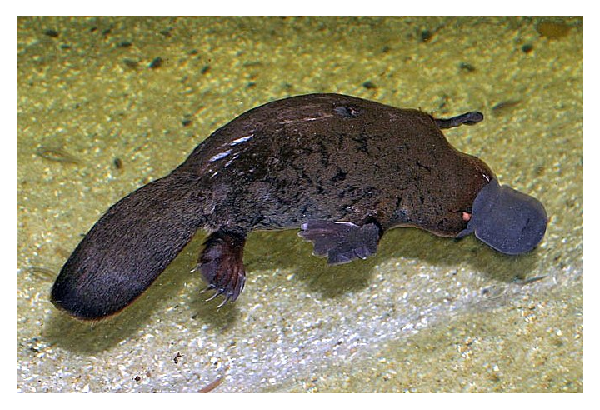
\includegraphics[width=45mm]{figs/Platypus.eps}
  	\end{column}
  	\begin{column}[T]{0.6\linewidth}
  	  \begin{itemize}
  	  	\item[\ding{51}]<3->{Has fur}
  	  	\item[\ding{51}]<4->{Has beak}
  	  	\item[\ding{51}]<5->{Lays eggs}
  	    \item[\ding{51}]<6->{Webbed feet}
  	    \item[\ding{51}]<7->{Feeds young with milk}
  	  \end{itemize}
  	\end{column}
  \end{columns}

\end{frame}

\begin{frame}[fragile]
  \frametitle{Multiple inheritance}
  
  \begin{columns}[t]
    \begin{column}[T]{0.49\linewidth}
  		Simple, just use multiple inheritance:
  		\begin{lstlisting}
class Platypus :
  public Mammal, public Bird,
  public Amphibian
{
public:
  void stingWithSpur();
};
  		\end{lstlisting}
  		So \texttt{Platypus} gets everything from \texttt{Mammal}, \texttt{Bird} and \texttt{Amphibian}.
  	\end{column}
  	\pause
  	\begin{column}[T]{0.49\linewidth}
	  	But wait.  A platypus can't fly! \pause{}  Okay, so let's override \texttt{fly} and make it private:
		  \begin{lstlisting}
class Platypus :
  public Mammal, public Bird,
  public Amphibian
{
public:
  void stingWithSpur();
private:
  void fly();
};
  		\end{lstlisting}  
  	\end{column}
  \end{columns}
  \pause
  		Now if you try to do this:
  		\begin{lstlisting}[belowskip=0pt]
int main()
{
  Platypus platypus;
  platypus.fly(); // Compiler error: can't access private!
  return 0;
}
  		\end{lstlisting}
  

\end{frame}

\section{Polymorphism}

\subsection{Huh.  What is it good for?}

\begin{frame}[fragile]
  \frametitle{Polymorphism}
  \framesubtitle{The solution to all your animal taxonomy needs}

	Let's bring Fido back out.  What happens when we try:
  \begin{columns}[t]
    \begin{column}[T]{0.48\linewidth}
  		\begin{lstlisting}[aboveskip=0pt]
int main()
{
  Dog fido(2, 10,
    "Boston terrier");
    
  // Perfectly valid, after
  // all a Dog is a mammal:  
  Mammal * fidoPtr = &fido;
  fidoPtr->speak();

  return 0;
}
  		\end{lstlisting}
  	\end{column}
  	\pause
  	\begin{column}[T]{0.48\linewidth}
  		\cout{Grrrr, mammal noise!}
  	\end{column}
  \end{columns}
  \pause
  Huh?  Why is Fido speaking like a mammal again?

\end{frame}

\begin{frame}[fragile]
  \frametitle{Virtual functions}
  
  Virtual functions provide the solution:
  \begin{columns}[t]
    \begin{column}[T]{0.48\linewidth}
			\lstinputlisting[language=C++,%
    		title=\lstsrctitle,aboveskip=0pt,
    		linerange={4-5,14-15,19-19,54-55,63-64,67-67,85-89}]%
    		{../code/5_advanced_oop/lectures/virtual_functions.cpp}
    \end{column}
    \pause
		\begin{column}[T]{0.48\linewidth}
			\lstinputlisting[language=C++,%
    		aboveskip=0pt,belowskip=0pt,
    		linerange={91-99}]%
    		{../code/5_advanced_oop/lectures/virtual_functions.cpp}
    	\cout{Woof!}
		\end{column}
	\end{columns}
	\pause
	As if by magic, the correct method in \texttt{Dog} gets called.  This works for multiply derived types if they all use the \kw{virtual} keyword.

\end{frame}

\begin{frame}[fragile]
  \frametitle{Virtual functions}
  \framesubtitle{Health warning}
  
  \warnblock{If you declare any of your methods to be \kw{virtual} make sure to have a \kw{virtual} destructor!\newline
  Otherwise your object will not be destructed properly!}

\end{frame}

\subsection{Abstract base classes}

\begin{frame}[fragile]
  \frametitle{Abstract base classes}
  \framesubtitle{I'll take one of  your finest mammals please}
  
  At the moment we can do this:
  \begin{columns}[t]
    \begin{column}[T]{0.48\linewidth}
  		\begin{lstlisting}[aboveskip=0pt]
int main()
{
  Mammal theFinest(27, 70);
  
  theFinest.speak();
  
  return 0;
}
			\end{lstlisting}
		\end{column}
		\begin{column}[T]{0.48\linewidth}
		  \cout{Grrrr, mammal noise!}
		\end{column}
	\end{columns}
	But this doesn't make a lot of sense.  A mammal is an abstraction, we shouldn't be able to instantiate a concrete mammal.  We just want all derived types to be able to speak.

\end{frame}

\begin{frame}[fragile]
  \frametitle{Abstract base classes}
  
  The solution: use a pure virtual function by adding \texttt{ = 0}.
	\lstinputlisting[language=C++,%
  	title=\lstsrctitle,
  	linerange={4-5,14-15,19-19,90-96}]%
  	{../code/5_advanced_oop/lectures/pure_virtual_functions.cpp}
  	\pause
  Now \texttt{Mammal} is deemed to be abstract and cannot be instantiated but any concrete derived type that we do want to instantiate needs to be able to speak or do whatever it is that mammals do. Perfect.

\end{frame}

\subsection{Real world example}

\begin{frame}[fragile]
  \frametitle{Abstract bases classes example}
  \framesubtitle{Back to the real world}
  We want to write a log of how our simulation is progressing, but it may be convenient to be able to log to the screen, to file or to a database.
  \begin{lstlisting}[basicstyle=\ttfamily\fontsize{7}{8}\selectfont]
class Logger {
  virtual void logMessage(const std::string & message) = 0;
  virtual ~Logger() {}
};

class ScreenLogger : public Logger {
  virtual void logMessage(const std::string & message);
};

class FileLogger : public Logger {
  virtual void logMessage(const std::string & message);
};

class DatabaseLogger : public Logger {
  virtual void logMessage(const std::string & message);
};

int main()
{
  Logger * myLogger = new FileLogger("program.log");
  myLogger->writeMessage("Hello universe!")
  return 0;
}
  \end{lstlisting}

\end{frame}


\section{Friendship}

\subsection{Friend functions}

\begin{frame}[fragile]
  \frametitle{Friend functions}
  %\framesubtitle{I only give friends access to my privates}
  
  We've seen that only a class can access its \kw{private} members.  Sometimes we may want to make an exception for a particular external function.  We do this with the \kw{friend} keyword followed by the function prototype:
  \pause
  \lstinputlisting[language=C++,%
    basicstyle=\ttfamily\fontsize{8}{9}\selectfont,%
    title=\lstsrctitle,belowskip=0pt,
    linerange={3-13,31-34}]%
    {../code/5_advanced_oop/lectures/friend_function.cpp}

\end{frame}

\begin{frame}[fragile]
  \frametitle{Friend functions}
  \framesubtitle{Not for every day}
  
  \warnblock{
  	\begin{itemize}
  	\item The use of \kw{friend}s can undermine encapsulation, after all you're giving away access to parts of your class that were designed to be kept internal.
  \pause
  \item Sometimes friendship can be used effectively to keep dependent code separated if there is a good design reason.  For example the code to draw a rectangle may be very complicated and may fit more naturally in the graphics handling portion of the codebase.  This enhances encapsulation.
	\end{itemize}
  }

\end{frame}


\subsection{Friend classes}

\begin{frame}[fragile]
  \frametitle{Friend classes}
  \framesubtitle{Not a taxonomy of friends}
  
  We can grant \kw{friend} status to an entire class:
  \begin{lstlisting}
  class SolarSystem {
  private:
    Vector2 planetPositions[NUM_PLANETS];
    Planet planets[NUM_PLANETS];
    friend class Planet;
  };
  
  class Planet {
  public:
    Vector2 getPosition()
    { return mySystem.planetPositions[myIndex]; }
  private:
    unsigned int myIndex;
    SolarSystem & mySystem;
  };
  \end{lstlisting}
  \pause
  Friend classes can be useful in highly coupled parts of code like this: a \texttt{Planet} cannot exist without a \texttt{SolarSystem}.
  
\end{frame}

\subsection{Friendship non-transitivity}

\begin{frame}
  \frametitle{Friendship rules}
  \framesubtitle{Let's define some ground rules}
  
  The following transitivity and reciprocity rules apply to the \kw{friend} property:
  \begin{itemize}
  	\item{Friendship isn't reciprocated: Just because a friend can access a classes \kw{private} members doesn't mean the class can access the friend's.  It has to be explicitly marked as a \kw{friend}.}\pause
  	\item{Friendship isn't transitive: Friends of a friend can't access a classes \kw{private} members.}\pause
    \item{Friendship isn't inherited:  Friends can't access derived classes \kw{private} members.}
  \end{itemize}
  \pause Also note classes aren't automatically friends of their derived classes.

\end{frame}  
\begin{frame}
	\begin{center}
		\Large{Thank You!}
	\end{center}
\end{frame}
\end{document}